\section{Задание 1}

Настройка рабочей среды:
\begin{enumerate}
	\item Установить дату начала проекта - первый понедельник 2-го квартала текущего года \ref{fig:1};
	\item Установить длительность работы в днях, объем работы в часах, тип задач - с фиксированной длительностью \ref{fig:1};
	\item Установить стандартный календарь рабочего времени \ref{fig:2} \ref{fig:3};
	\item Учесть празники, попадающие на период реализации проета \ref{fig:4}.
\end{enumerate}
\begin{figure}[H]
	\centering
	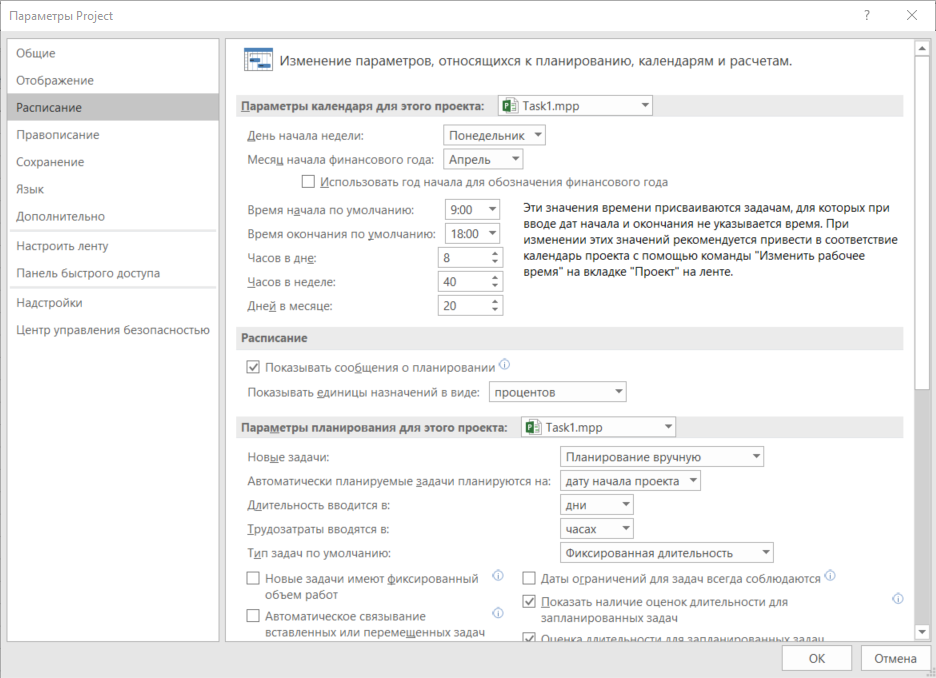
\includegraphics[width=0.7\linewidth]{src/1}
	\caption{Настройка среды проекта}
	\label{fig:1}
\end{figure}
\begin{figure}[H]
	\centering
	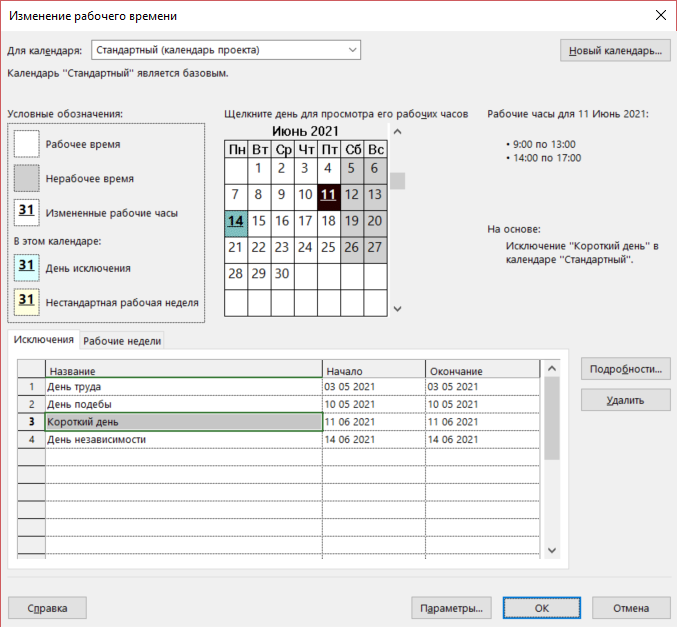
\includegraphics[width=0.7\linewidth]{src/2}
	\caption{Выходные дни}
	\label{fig:2}
\end{figure}
\begin{figure}[H]
	\centering
	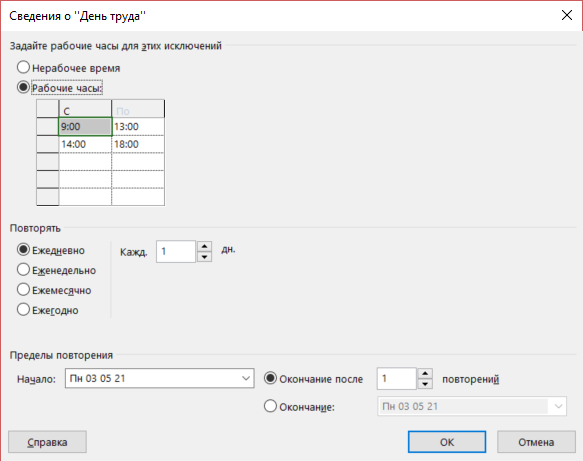
\includegraphics[width=0.7\linewidth]{src/3}
	\caption{Время работы}
	\label{fig:3}
\end{figure}
\begin{figure}[H]
	\centering
	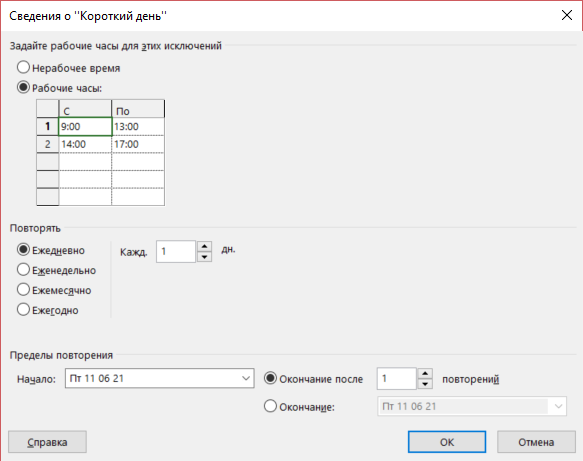
\includegraphics[width=0.7\linewidth]{src/4}
	\caption{Короткий день}
	\label{fig:4}
\end{figure}

\section{Задание 2}
Создание списка задач \ref{fig:5}
\begin{figure}[H]
	\centering
	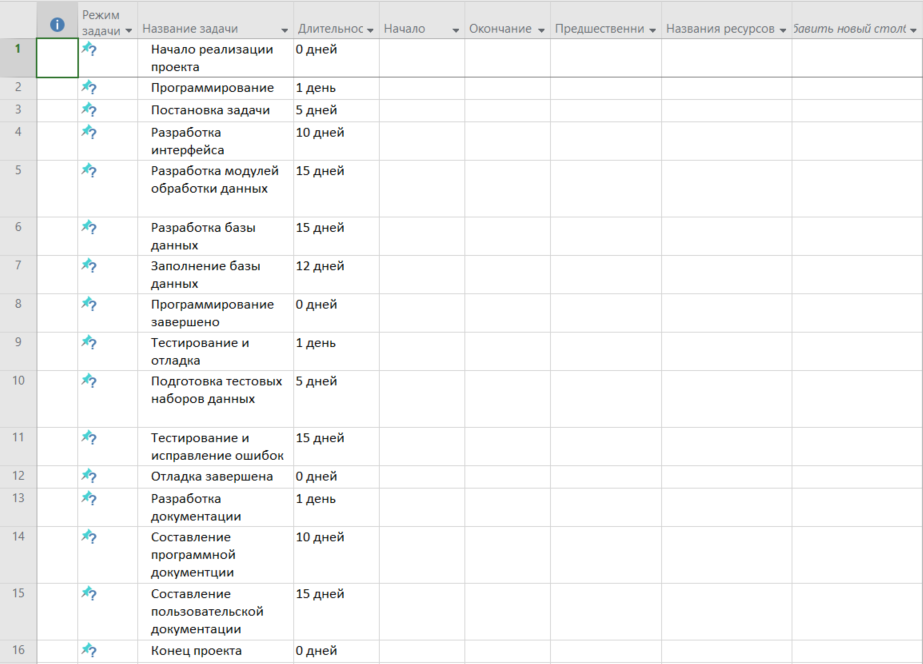
\includegraphics[width=0.7\linewidth]{src/5}
	\caption{Список задач}
	\label{fig:5}
\end{figure}

\section{Задание 3}
Структурирование списка задач \ref{fig:6}
\begin{figure}[H]
	\centering
	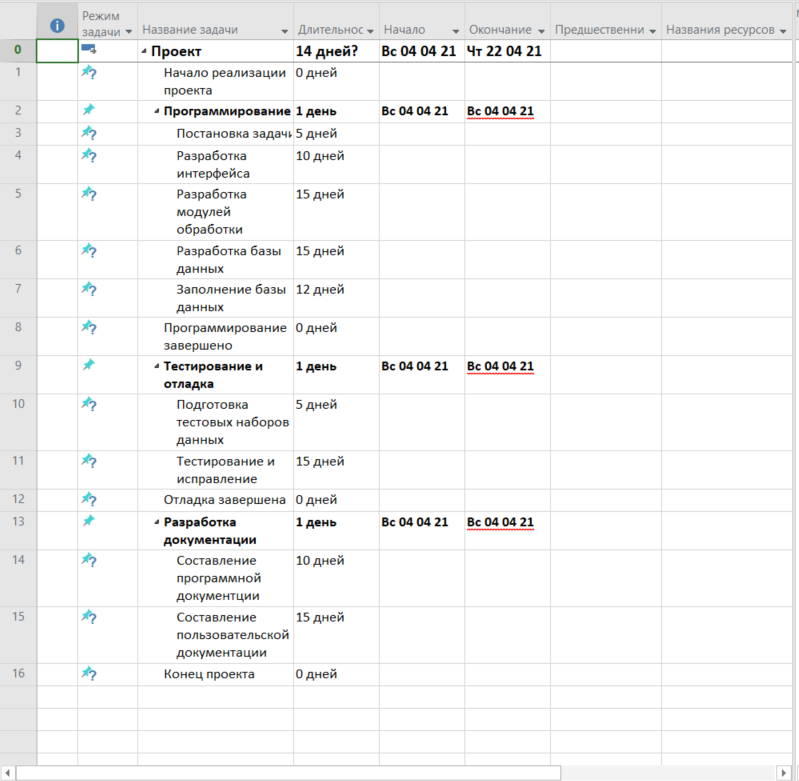
\includegraphics[width=0.7\linewidth]{src/6}
	\caption{Структурированный список задач}
	\label{fig:6}
\end{figure}

\section{Задание 4}
Установление связей между задачами\ref{fig:7}
\begin{figure}[H]
	\centering
	
\includegraphics[width=0.7\linewidth]{src/7}
	\caption{Связанные задачи}
	\label{fig:7}
\end{figure}

В данный момент продолжительсность проекта составляет 68 дней. Что полностью укладывается в рамки проекта по времени.

\section{Задание 5}
Создание списка ресурсов \ref{fig:8}
\begin{figure}[H]
	\centering
	
\includegraphics[width=0.7\linewidth]{src/8}
	\caption{Список ресурсов}
	\label{fig:8}
\end{figure}

\section{Задание 6}
Назначение ресурсов задачам \ref{fig:9}.
Назначение фикс. трат \ref{fig:10}
\begin{figure}[H]
	\centering
	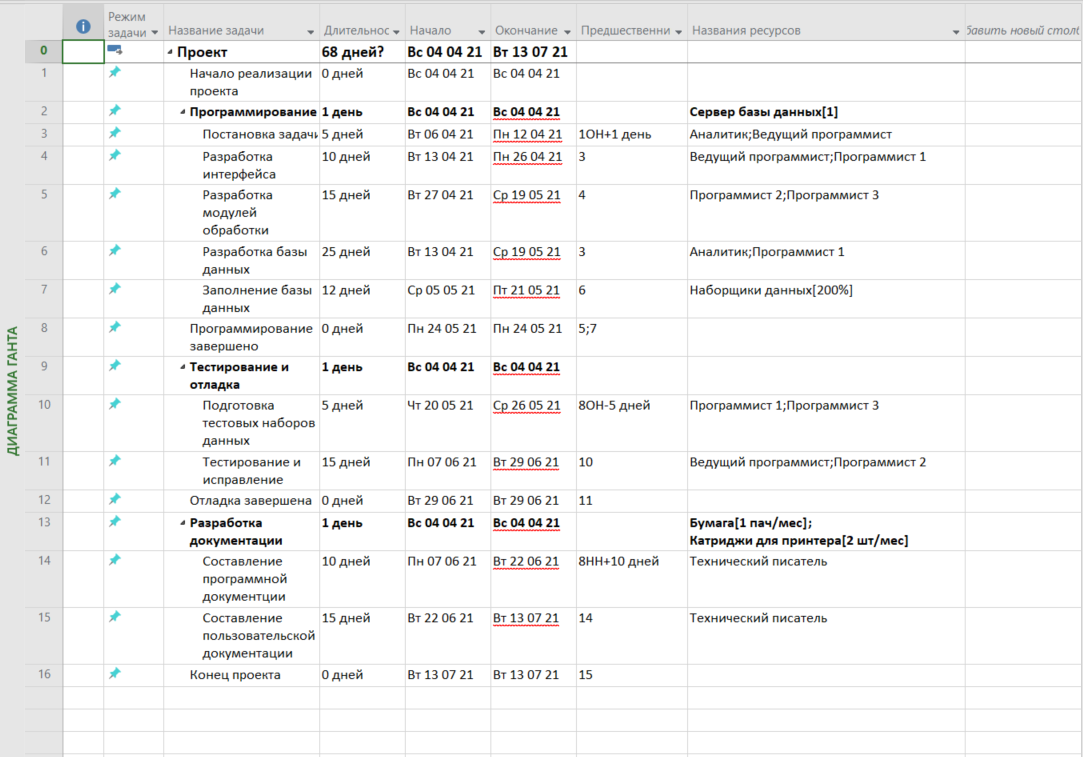
\includegraphics[width=0.7\linewidth]{src/9}
	\caption{Назначение ресурсов задачам}
	\label{fig:9}
\end{figure}
\begin{figure}[H]
	\centering
	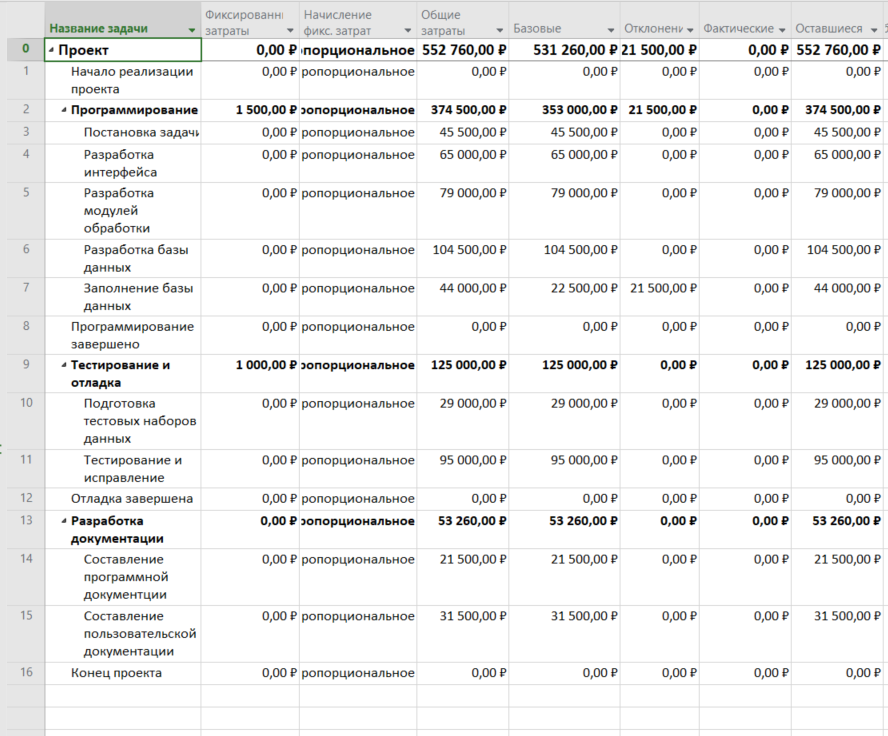
\includegraphics[width=0.7\linewidth]{src/10}
	\caption{Назначение фиксированных трат}
	\label{fig:10}
\end{figure}

В данный момент стоимость проекта составляет 552760рублей что укладывается в проект.

\section{Задание 7}
Утсранить перегрузку ресурсов.
В данной работе отсутсвует перегрузка ресурсов.

\section{Задание 8}
После добавления профилактики стоимость 3000р за каждый вызов стоимость проекта составила 577 097р.
Для того что бы другие задачи на выполнялись в момент профилактики, поменяем тип задач и нагрузим профилактику всеми ресурсами.
Потом удалим \ref{fig:13}
\begin{figure}[H]
	\centering
	
\includegraphics[width=0.7\linewidth]{src/13}
	\caption{Отдых во время профилактики}
	\label{fig:13}
\end{figure}























